\section{Solution Architecture}
\label{sec:solution_architecture}
Actually a typical scenario for an IoT application consists of a smart space that contains several smart objects and all
the infrastructure required to support this application, namelly RIFD tags, sensors, readers and servers, as illustrated at the
Figure \ref{fig:smart-space}. This scenario presents several issues regarding the deployment of the application, the low scalability, the costs of infrastructure
and the maintenance of the same.
% Typical Smart Space Scenario
\begin{figure}[h!]
  \centering
  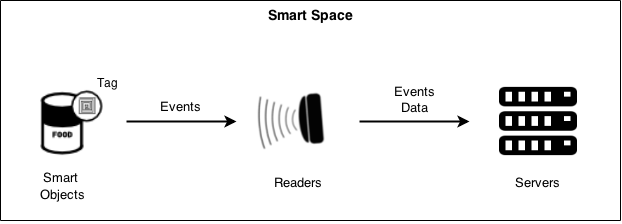
\includegraphics[width=\textwidth]{./images/smart-space}
  \caption{Typical smart space scenario.}
  \label{fig:smart-space}
\end{figure}\\
By converging the IoT applications with the Cloud Computing paradigm the objective is simplify this scenario by leveraging the required infrastructure by these applications to the Cloud providers,
as illustrated at the Figure \ref{fig:smart-space-cloud}. Furthermore, the convergence of this two paradigms, allows to take advantage of the benefits offered by Cloud computing as referenced
in \textbf{Section \ref{sub:cloud_computing}}.
% Cloud-based Smart Space Scenario
\begin{figure}
  \centering
  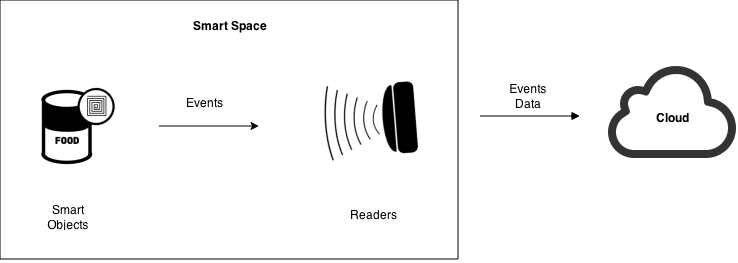
\includegraphics[width=\textwidth]{./images/smart-space-cloud}
  \caption{Cloud-based smart space.}
  \label{fig:smart-space-cloud}
\end{figure}\\
% -----------------------------------------------
% STATE OF ART
% -----------------------------------------------
\subsection{State of Art}
\label{sub:state_of_art}
Actually Cloud-based IoT applications are the state of art of this kind of solutions. By leveraging the infrastructure to the Cloud providers, these applications has a high-availabity, can dinamically scale
while spending a fraction compared with the tradional solutions. However, as earlier mentioned the deployment of such applications still is an issue, due its complexity and required manual intervention. The
deployment of Cloud-based IoT applications usually are performed through IT automation tools, such as Chef\footnote{www.chef.io} and Puppet\footnote{puppetlabs.com}. These tools enables to automate the deployment
of such applications in a certain way, given that all the components of the application and the relation between themselves must be specified manually, which requires considerable manual work and expertise by
the person that is performing the deployment. However, the deployment process of these solutions is not the only existent issue. Monitoring the application life-cycle is a task that requires a lot of effort and expertise
by the system admnistrators.\\

In order to solve this problem, the adopted approach relies on perform the deployment of these applications by using Cloud Orchestrator tools. As mentioned in \textbf{Section \ref{sub:cloud_orchestration}}, these
tools allows to specify the application components and their relations in a high-level perspective and to execute the management tasks required by the application during its life-cycle.
As a matter of fact, in a low-level perspective cloud orchestration tools express the high-level perspective defined by the user into scripts that latter are executed using IT automation tools such as Puppet and Chef.
% -----------------------------------------------
% CLOUD OF THINGS ARCHITECTURE
% -----------------------------------------------
\subsection{Cloud of Things Architecture}
\label{sub:cloud_of_things_architecture}
The main objective of Cloud of Things decrease the complexity of deployment and management of IoT applications. To achieve this objective, Cloud of Things must enable non-technical users - the business managers - to perform the
monitoring of Cloud-based IoT applications as well defining Service Level Agreements in a high-level way. In order execute this tasks, users must be able to interact with the application that is running at the cloud in order
to observe their state and to apply some decisions based on the performance of the application. Thus, Cloud of Things must provide a service that allows the users to perform such actions. At Figure \ref{fig:cloud_of_things_architecture}
we present the Cloud of Things architecture.
\vspace{1in}
% Cloud of Things Architeture
\begin{figure}[h!]
  \centering
  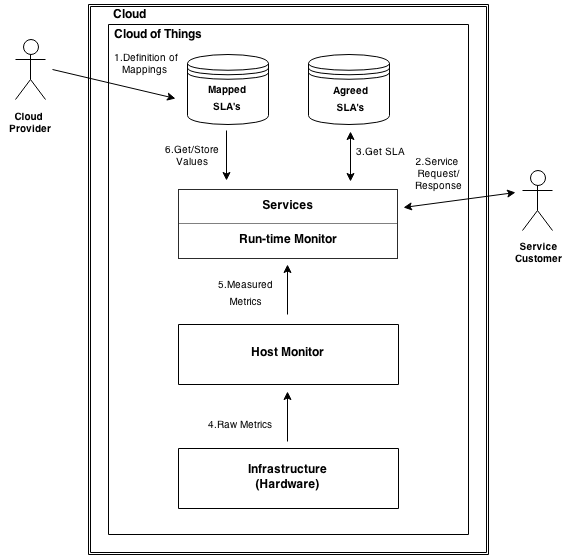
\includegraphics[width=.8\textwidth]{./images/cloud-of-things-architecture}
  \caption{Cloud of Things Architecture.}
  \label{fig:cloud_of_things_architecture}
\end{figure}\\
The presented architecture is based on the LoM2HiS Framework \cite{emeakaroha2010low} architecture. In this architecture the \textit{Services} component and the \textit{Run-time Monitor} represents the application layer where services are
deployed using a Web Service container. The \textit{Run-time Monitor} is responsible to monitor the services based on the negotiated and agreed SLAs. After the Cloud provider agrees on the SLA terms, the agreed SLAs are stored in the repository for
service provisioning and the following steps are executed:
\begin{enumerate}
  \item The Cloud provider creates rules for the framework mappings using Domain Specific Languages\footnote{Domain Specific Languages are small languages that normally are tailored to a specific problem domain.} (DSL's).
  \item The customer requests the provisioning of an agreed service.
  \item Once the request is received, the run-time monitor loads the service SLA from the agreed SLA repository.
  \item The resource metrics are measured by monitoring agents, these metrics are stored in a raw format that later are accessed by the host monitor.
  \item The host monitor extracts metric-value pairs from the raw metrics and them transmits them periodically to the run-time monitor.
  \item After receive the low-level metrics, the run-time monitor uses predefined mapping rules to map the low-level metrics into a equivalent form of the agreed SLA and them the resulting map is stored in the mapped metrics repository.
\end{enumerate}\\
In this architecture, the \textit{Run-time monitor} uses the mapped values to monitor the status of the deployed services. Once it detects that a SLA is violated, the \textit{Run-time monitor} must alert the customer of the violated SLA.
At this point the customer is responsible to take the decisions in order to correct the state of the system.
